Um escoamento monofásico, permanente e plenamente desenvolvido
de um fluido newtoniano e incompressível 
entre placas horizontais paralelas onde a placa inferior se desloca com velocidade \textit{$U_{bottom}$}
enquanto a placa superior se desloca com velocidade \textit{$U_{top}$} é 
conhecido como \textit{Escoamento de Couette}.
A \ref{couette} apresenta esquematicamente este escoamento e
o perfil do campo de velocidade esperado.

\begin{figure}[H]
\begin{center}
\begin{tikzpicture}[scale=1.2]
 \draw [pattern=north east lines] (0,0) -- (0,-0.1) -- (5,-0.1) -- (5,0) -- cycle;
 \draw [pattern=north east lines] (0,1) -- (0,1.1) -- (5,1.1) -- (5,1) -- cycle;

 \draw [->,thick] (5.1,1)--(6,1) node[above] {$U_{top}$};
 \draw [->,thick] (-0.1,0)--(-1,0) node[below] {$U_{bottom}$};
 
 \draw [->,thick] (-4,-0.1)--(-4,1.5) node[left] {$y$};
 \draw [->,thick] (-4.1,0)--(-2.5,0) node[below] {$x$};
 
 \draw [dotted] (2.5,0.0) to (2.5,1.0);
 \draw  (1.5,0.0) to (3.5,1.0);
 
 \draw [->,thick] (2.5,0.0) to (1.5,0.0);
 \draw [->,thick] (2.5,0.15) to (1.8,0.15);
 \draw [->,thick] (2.5,0.35) to (2.2,0.35);

 \draw [->,thick] (2.5,1) to (3.5,1);
 \draw [->,thick] (2.5,0.85) to (3.2,0.85);
 \draw [->,thick] (2.5,0.65) to (2.8,0.65);
\end{tikzpicture}
\end{center}
\caption{Escoamento de Couette}
\label{couette}
\end{figure}


\noindent
O perfil de velocidade que este escoamento adquire 
é dado pela equação abaixo:

\begin{equation}
 u = \big[ U_{top} - U_{bottom} \big] \frac{y}{L} + U_{bottom}
\end{equation}

\medskip
\noindent
onde $U_{top}$ é a velocidade que a placa superior se desloca e seu valor é
$U_{top} = 1$, 
$U_{bottom}$ é a velocidade que a placa inferior se desloca e seu valor é
$U_{bottom} = -1$, 
$L$ é a largura não dimensional
entre as placas e seu valor é $L = 1$
e $y$ é a distância entre as placas e varia entre $y = \big[ 0,1 \big]$.
O domínio foi discretizado utilizando uma malha 
triangular linear com 3835 nós e 7299 elementos. 

\medskip
\noindent
As condições de contorno utilizadas foram:

\begin{itemize}
     \item \textit{condição de entrada}: nenhum valor é especificado. As derivadas das
      componentes tangencial e normal da velocidade e da função de corrente possuem o 
      valor nulo, isto é,
      $\partial u/\partial n = 0$,
      $\partial v/\partial n = 0$ e
      $\partial \psi/\partial n = 0$ respectivamente.

     \item \textit{condição de movimentação da parede}: esta condição é utilizada na placa superior e inferior, 
      onde todas as componentes da velocidade e da função de corrente são especificadas.
      Para a parede superior, $u=U_{top}$, $v=0$ e $\psi=0$, onde $U_{top} = 1$.
      Para a parede inferior, $u=U_{bottom}$, $v=0$ e $\psi=0$, onde $U_{bottom} = -1$.

     \item \textit{condição de saída}: assim como na entrada, nenhum valor é especificado. As derivadas das
      componentes tangencial e normal da velocidade e da função de corrente possuem o 
      valor nulo, isto é,
      $\partial u/\partial n = 0$,
      $\partial v/\partial n = 0$ e
      $\partial \psi/\partial n = 0$ respectivamente.
\end{itemize}


\newpage
A \ref{velocidade couette} apresenta a evolução 
do perfil de velocidade no tempo quando o $Re=100$, além do comparativo
entre a solução numérica e a solução analítica no estado permanente do
problema proposto. É possível observar que a solução numérica converge
para a solução analítica quando o escoamento torna-se permanente.


\begin{figure}[H]
     \centering
     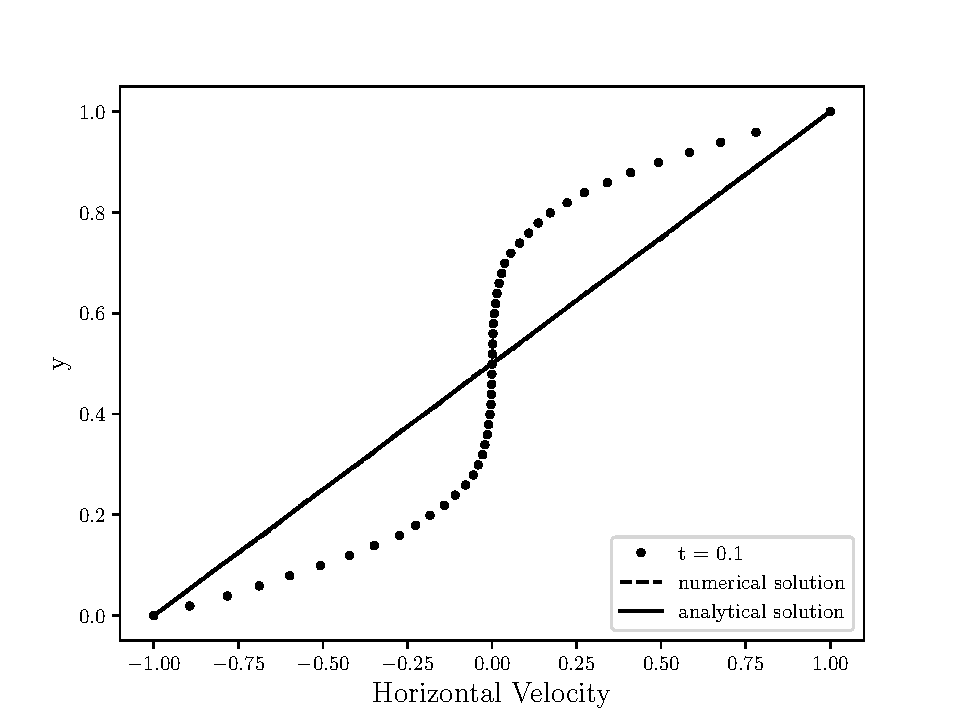
\includegraphics[scale=1]{./02_chaps/cap_validation/figure/couette_velocity.pdf}\\
     \medskip
     \caption{Evolução do perfil de velocidade no tempo para $Re=100$ e
     a comparação da solução numérica com a solução analítica para o Escoamento de Couette.}
     \label{velocidade couette}
\end{figure}

\newpage
